\capitulo{5}{Aspectos relevantes del desarrollo del proyecto}



\section{Introducción}
En este capítulo se recogen los aspectos más interesantes del desarrollo del proyecto, donde se documenta desde la metodología aplicada para el desarrollo del proyecto, describiendo los pasos a seguir y el alcance que se espera que tenga el proyecto. Por otro lado, también se detalla la planificación del proyecto, cuál es el modelo de los datos, qué operaciones de transformación y limpieza han sido necesarias y finalmente se describe cómo se ha implementado el proyecto describiendo los archivos y carpetas que forman parte del proyecto.


\section{Metodología}
La metodología de este proyecto tiene como base un enfoque que comprende varias etapas clave. En primer lugar, se realizará una revisión de diferentes artículos sobre técnicas de inteligencia artificial aplicadas al análisis de datos deportivos, centrándose especialmente en la predicción del rendimiento de equipos de fútbol basándose en la rotación de los jugadores. Esta revisión ayudará a identificar las mejores prácticas y los enfoques que pueden ser más relevantes para el desarrollo del proyecto.

Entre estos artículos analizados destaca (Ondrej Hubácek, Gustav Sourek, Filip Zelezný, 2019 \cite{rusos}) donde utiliza \textit{gradient boosted trees} para intentar predecir el ganador del partido. Para ello, sobre un conjunto de datos con 200.000 registros, experimentan con métodos relacionales y basados en características denominados ``RDN-Boost'' y ``Xgboost''. Por otro lado, utilizan \textit{pi-ratings} que capturan tanto la forma actual como las fortalezas históricas de los equipos.

También destaca (Julian Knoll, Johannes Stübinger, 2019 \cite{alemanes}) donde usando algoritmos de \textit{machine learning} intentan predecir el resultado de los partidos. En este trabajo utilizan diferentes variables como las relacionadas con la efectividad de la defensa y ataque de los equipos. Los algoritmos que utiliza son SVM, bosques aleatorios y \textit{boosting}.

Por otro lado, en (Igiri, Chinwe Peace, Nwachukwu, Enoch Okechukwu, 2014 \cite{africanos}) implementan un sistema de predicción de resultados de partidos de fútbol utilizando técnicas de redes neuronales artificiales y regresión logística. Los resultados de este trabajo muestran que los modelos creados tienen una alta precisión en comparación con los sistemas previos.

En el trabajo de (Nilay Zaveri, Utkarsh Shah, Shubham Tiwari, Pramila Shinde, Lalit Kumar Teli, 2018 \cite{indios}) utilizan algoritmos de \textit{machine learning} para predecir partidos de fútbol, considerando únicamente equipos de LaLiga española en las últimas cinco temporadas. Para el análisis, utilizan estadísticas de jugadores y equipos del juego FIFA 18. Finalmente, proponen un sistema que sugiere tácticas para maximizar las probabilidades de victoria de un equipo.

Finalmente en (Juan Diego Fernández García, 2019 \cite{tfg-laguna}) utiliza modelos probabilísticos para la estimación de resultados deportivos utilizando la distribución de Poisson. En el primer modelo asume independencia entre los goles que anotan los equipos y el segundo modelo, con Poisson Bivariante, asume correlación entre el número de goles de ambos equipos.



Posteriormente, se llevará a cabo la recopilación y preparación de datos, donde se recogerán conjuntos de datos históricos que abarquen información relevante sobre la rotación de jugadores y el rendimiento deportivo de equipos de fútbol en las ligas seleccionadas. Esta etapa incluye la limpieza de datos, la preparación de los datos para su análisis posterior y un breve análisis sobre ellos para detectar patrones.

Una vez preparados los datos, se realizará la implementación y evaluación de modelos de inteligencia artificial. Se probarán los diferentes algoritmos comentados en la parte teórica y diferentes redes neuronales utilizando los parámetros también comentados. Los modelos se entrenarán y ajustarán utilizando los datos que se han obtenido previamente y se evaluará su rendimiento utilizando las métricas enumeradas en la parte teórica. Esta fase permitirá detectar los modelos más eficaces y precisos para predecir el rendimiento deportivo basado en la rotación de jugadores.

Finalmente, se tratará de optimizar al máximo el rendimiento de los mejores modelos seleccionados buscando los parámetros que hagan que estos modelos tengan mejores valores en las métricas seleccionadas y de esta manera sean más precisos y puedan ayudar a los directivos en la toma de decisiones sobre las estrategias de gestión de jugadores.

\section{Alcance}
El alcance de este proyecto abarca la evaluación y aplicación de diversas técnicas de inteligencia artificial para predecir el rendimiento de equipos de fútbol basándose en la rotación de jugadores. En primer lugar, después de definir la metodología, se seleccionarán las técnicas más correctas para el análisis de datos relacionados con la rotación de jugadores y el rendimiento deportivo. Este apartado incluirá la recopilación, preprocesamiento y análisis de los datos de las ligas, equipos y jugadores de fútbol seleccionados. Para la parte del análisis de los datos, se realizan unos pequeños programas que analicen los datos obtenidos mediante mapas de calor para poder detectar patrones. Al detectar estos patrones se pretende justificar si las estrategias de rotación aplicadas por los equipos mejoran el rendimiento o no.

Las ligas sobre las que se obtendrán y utilizarán los datos serán LaLiga EA Sports (primera división española), Premier League (primera división inglesa) y Bundesliga (primera división alemana) desde la temporada 2018/2019 hasta la temporada 2023/2024, ambas incluidas. Esta
variedad en la elección de ligas y temporadas permite evaluar si existen diferencias significativas
entre las ligas de los diferentes países o entre las temporadas. Otra ventaja es que al utilizar datos de diferentes ligas y temporadas, probablemente los modelos creados sean más robutos y tengan mayor capacidad de generalización.

Además, el alcance del proyecto se pretende que también implique la implementación y ajuste de modelos de inteligencia artificial para la predicción del rendimiento deportivo en función de la rotación de jugadores. Para ello, se explorarán diversas técnicas de inteligencia artificial y \textit{machine learning}, como redes neuronales, árboles de decisión y métodos de aprendizaje automático supervisado, con el objetivo de detectar aquellas que mejor se adapten a las características de este problema. Sobre cada una de ellas, se realizará una optimización de parámetros para mejorar todo lo posible su precisión.

Finalmente, se realizará una evaluación de los modelos desarrollados, utilizando métricas de rendimiento para definir su calidad en la predicción del rendimiento de los equipos. Después de esto, se seleccionarán los mejores modelos.

Se pretenden obtener tres modelos, uno entrenado para predecir el ganador del partido, otro para predecir el número de goles que anotará el equipo local y otro para predecir el número de goles que anotará el equipo visitante. 

Es cierto que se pretenden obtener los modelos lo más precisos posibles y que realicen las mejores predicciones, pero sin embargo, el objetivo principal del proyecto es determinar qué estrategias y qué acciones sobre la gestión de los jugadores contribuyen al mejor rendimiento de los equipos de fútbol. Por lo tanto, no se debe desviar el foco y plantear que los modelos sean capaces de realizar predicciones exactas sobre los partidos, ya que por un lado, este no es el objetivo y por otro lado, esto es algo bastante complejo debido a la incertidumbre que hay en cada partido de fútbol y la aleatoriedad que rodea cada evento de este tipo.

Además de todos estos aspectos comentados, se documentarán y analizarán todas las tareas realizadas en el proyecto, con el objetivo de ofrecer recomendaciones para la gestión de la rotación de jugadores en equipos de fútbol, así como posibles áreas de mejora y futuras investigaciones para este proyecto.




\section{Plan de proyecto}

El proyecto comienza las primeras semanas durante la estancia en un GIR para la asignatura de I+D+i donde se realiza una parte de investigación y se desarrolla el núcleo del proyecto. Para finalizar, el proyecto continua como Trabajo de Fin de Máster, donde se sigue profundizando y expandiendo el trabajo realizado previamente. La duración de cada una de estas secciones es 190 horas y 150 horas respectivamente, sumando en total 340 horas. La fecha de inicio del proyecto es el 29 de abril de 2024 y la fecha límite de finalización es el 28 de junio de 2024.


La Tabla \ref{table:planificacion} muestra la planificación de las semanas durante las que se desarrolla el proyecto.

\begin{table}[]
    \centering
    \begin{tabular}{|c|c|c|c|c|}
        \hline
        { \textbf{Semana}} & { \textbf{Fecha de inicio}} & { \textbf{Fecha de fin}} & { \textbf{Carga de trabajo}} & { \textbf{Sección}} \\ \hline
        1                  & 29/04/2024                  & 05/05/2024               & 40 horas                     & I+D+i               \\ \hline
        2                  & 06/05/2024                  & 12/05/2024               & 40 horas                     & I+D+i               \\ \hline
        3                  & 13/05/2024                  & 19/05/2024               & 40 horas                     & I+D+i               \\ \hline
        4                  & 20/05/2024                  & 26/05/2024               & 30 horas                     & I+D+i               \\ \hline
        5                  & 27/05/2024                  & 02/06/2024               & 24 horas                     & I+D+i               \\ \hline
        6                  & 03/06/2024                  & 09/06/2024               & 16 horas                     & I+D+i               \\ \hline
        7                  & 10/06/2024                  & 16/06/2024               & 60 horas                     & TFM                 \\ \hline
        8                  & 17/06/2024                  & 23/06/2024               & 60 horas                     & TFM                 \\ \hline
        9                  & 24/06/2024                  & 28/06/2024               & 30 horas                     & TFM                 \\ \hline
    \end{tabular}
    \caption{Planificación de las semanas.}
    \label{table:planificacion}
\end{table}

En este proyecto se ha aplicado \textit{Scrum} desde el inicio. \textit{Scrum} es un marco ágil de gestión de proyectos que se aplica para desarrollar, entregar y mantener productos complejos. Está basado en la colaboración, la flexibilidad y la entrega incremental de productos. Scrum se encarga de dividir el trabajo en ciclos cortos llamados \textit{sprints}, que suelen durar entre dos y cuatro semanas. Cada \textit{sprint} comienza con una reunión de planificación donde se define el trabajo que se realizará y termina con una revisión y retrospectiva para analizar el progreso y mejorar los procesos realizados. Los roles clave en Scrum incluyen el \textit{Product Owner}, que define y prioriza el trabajo que se debe realizar en el proyecto, el \textit{Scrum Master} que facilita el proceso y se encarga de eliminar los impedimentos que puedan aparecer, y el equipo de desarrollo, que es responsable de desarrollar y entregar el producto de forma incrementable \cite{scrum}.

En proyectos de ciencia de datos, como es el que se pretende realizar en este caso, \textit{Scrum} se aplica para gestionar el ciclo de vida del desarrollo de los modelos y el análisis. Durante cada \textit{sprint}, el equipo puede enfrentar tareas como la recolección y limpieza de datos, el desarrollo y entrenamiento de modelos y la validación de resultados. El \textit{Product Owner} en este contexto puede ser un especialista en datos que determina las prioridades basándose según los objetivos del proyecto que se han planteado conseguir, mientras que el \textit{Scrum Master} asegura que el equipo pueda trabajar de manera eficiente eliminando todos los obstáculos y facilitando la comunicación entre el equipo. Las revisiones y retrospectivas permiten ajustar rápidamente las estrategias basadas en los resultados que se han obtenido, garantizando que el proyecto se mantenga siempre alineado con las metas planteadas y pueda adaptarse a nuevas necesidades y requerimientos \cite{scrum-data-science}.

Para este proyecto se ha aplicado \textit{Scrum} pero con diversas adaptaciones para ajustarlo a la naturaleza del proyecto. El primer lugar, la duración de los \textit{sprints} ha sido de una semana según la planificación que se puede apreciar en la Tabla \ref{table:planificacion}. Por otra parte, el alumno que se ha encargado de desarrollar el proyecto ha cumplido los roles de \textit{Product Owner}, \textit{Scrum Master} y equipo de desarrollo. Finalmente, se han realizado reuniones de planificación antes de comenzar los \textit{sprints} donde se definía el trabajo a realizar y reuniones de revisión al finalizar los \textit{sprints} para revisar los resultados obtenidos y sugerir mejoras.


\section{Modelo de los datos}
Los datos obtenidos se asocian a diferentes entidades que están relacionadas entre sí y abarcan multitud de campos, por ello, es importante estructurarlos de la manera correcta para que puedan ser utilizados adecuadamente en el entrenamiento de los modelos. En la figura \ref{fig:modelo-datos} se puede apreciar el modelo de los datos y como se han almacenado de forma estructurada después de extraerlos mediante \textit{scraping}.

\begin{figure}
    \centering
    \begin{normalsize}
        \import{svg/}{modelo-datos1.pdf_tex}
    \end{normalsize}
    \caption{Modelo de datos.}
    \label{fig:modelo-datos}

\end{figure}

Como se puede ver, en el diagrama los atributos de la entidad ``IndicadoresEquipoPrepartidoModelo'' no están incorporados ya que contiene 174 atributos. Más adelante se describen estos atributos.

A continuación, se realiza una breve descripción de cada entidad:
\begin{itemize}
    \item \textbf{``Equipo'':} recoge la información de cada equipo en una determinada liga y temporada. Cada equipo se identifica con un id único.
    \item \textbf{``Jugador'':} recoge la información de cada jugador en una determinada liga y temporada.
          Cada jugador se identifica con un id único y se le relaciona con el equipo en el que juega.
    \item \textbf{``Partido'':} recoge la información de cada partido en una determinada liga y temporada. Cada
          partido se identifica con un id único y se le relaciona con los equipos que lo juegan.
    \item \textbf{``DatosJugadorPartido'':} recoge la información de un jugador en un determinado partido en
          una determinada liga y temporada. Cada elemento se identifica con un id único y se le
          relaciona con el jugador y el partido al que se asocia.
    \item \textbf{``DatosPartidoJugado'':} recoge la información de un partido jugado en una determinada liga
          y temporada. Cada elemento se identifica con un id único y se relaciona con el partido al
          que se asocia.
    \item \textbf{``IndicadoresEquipoPrepartidoModelo'':} recoge los indicadores de los equipos que juegan
          un partido en una determinada liga y temporada. Cada elemento se identifica con un id
          único y se relaciona con el partido al que se asocia.
\end{itemize}

\hypertarget{explicacion-indicadores}{Los elementos de la entidad ``IndicadoresEquipoPrepartidoModelo'' son los datos con los que se
entrenan los modelos. Los indicadores que se incluyen en esta identidad miden el desempeño
previo de los equipos antes del partido. Estos indicadores pueden ser en forma de porcentaje,
proporción o media y pueden tener en cuenta los partidos previos de los equipos de forma general
en la temporada actual, es decir, sin distinguir si el equipo jugaba como local o visitante, o de
forma específica, solo evaluando los partidos previos del equipo donde ha jugado en el mismo
ámbito como lo va a hacer en el partido actual. Por ejemplo, para el equipo local de un partido,
solo se tendrían en cuenta los partidos previos que ha jugado como local.}

Respecto a los indicadores creados, miden diferentes valores asociados a las victorias, goles,
cambios realizados, tarjetas… de los equipos. Estos indicadores definen como llegan los equipos
al partido y por lo tanto son las variables explicativas. Sobre los cambios realizados, se evalúan
entre otras cosas las proporciones de cada equipo de realizar cambios en unos determinados
intervalos de tiempo, las proporciones de cambios según las posiciones de los jugadores afectados
o las proporciones de cambios en la alineación inicial también por posiciones.

Existen tres tipos de indicadores, en forma de porcentaje, proporción o media. A continuación se detalla el cálculo de cada uno de ellos:
\begin{itemize}
    \item \textbf{Indicadores en forma de porcentaje:} estos indicadores se calculan midiendo en qué porcentaje sobre el total de partidos jugados que se evalúen, se cumple una determinada condición. Por ejemplo, para el cálculo del porcentaje de partidos perdidos del visitante en el sitio, se calcula el porcentaje de cuántos partidos ha perdido el visitante jugando como visitante sobre cuántos partidos ha jugado el visitante como visitante en total.
    \item \textbf{Indicadores en forma de proporción:} estos indicadores se realizan calculando la cuenta total de un dato dividiéndolos entre el número de partidos jugados que se evalúen. Por ejemplo, para el cálculo de la proporción de puntos del local en general, se acumulan todos los puntos que haya obtenido el local jugando como local y visitante, es decir en todos sus partidos de la temporada, y se divide este valor entre el número de partidos que ha jugado el local tanto como local y visitante, es decir el total de partidos.
    \item \textbf{Indicadores en forma de media:} estos indicadores se calculan realizando la media sobre los datos recogidos de un determinado parámetro. Por ejemplo para la media del minuto en la que el local realiza los cambios en general, se calcula la media sobre los valores de los minutos de todos los cambios que ha realizado el local en todos sus partidos, ya sea de local o de visitante.
\end{itemize}


Además, en cada uno de estos elementos de esta entidad se incluyen las variables a predecir que
son los goles de cada equipo y el ganador del partido.

A continuación, se describen todos los atributos de esta entidad ``IndicadoresEquipoPrepartidoModelo'' agrupándolos según del tipo que sean:

\begin{itemize}
    \item Atributos base: atributos descriptivos de cada registro.
          \begin{itemize}
              \item id indicadores equipo prepartido
              \item id partido
              \item jornada
          \end{itemize}
    \item Atributos sobre el ganador: atributos relacionados con los ganadores de los partidos que han jugado.
          \begin{itemize}
              \item porcentaje del local de partidos ganados en sitio
              \item porcentaje del local de partidos ganados en general
              \item porcentaje del local de partidos empatados en sitio
              \item porcentaje del local de partidos empatados en general
              \item porcentaje del local de partidos perdidos en sitio
              \item porcentaje del local de partidos perdidos en general
              \item porcentaje del visitante de partidos ganados en sitio
              \item porcentaje del visitante de partidos ganados en general
              \item porcentaje del visitante de partidos empatados en sitio
              \item porcentaje del visitante de partidos empatados en general
              \item porcentaje del visitante de partidos perdidos en sitio
              \item porcentaje del visitante de partidos perdidos en general
              \item proporción del local de puntos obtenidos en sitio
              \item proporción del local de puntos obtenidos en general
              \item proporción del visitante de puntos obtenidos en sitio
              \item proporción del visitante de puntos obtenidos en general
          \end{itemize}
    \item Atributos sobre la cantidad de goles: atributos relacionados con la cantidad de goles totales de los partidos que han jugado.
          \begin{itemize}
              \item porcentaje del local de partidos con más 1,5 goles en sitio
              \item porcentaje del local de partidos con más 1,5 goles en general
              \item porcentaje del visitante de partidos con más 1,5 goles en sitio
              \item porcentaje del visitante de partidos con más 1,5 goles en general
              \item porcentaje del local de partidos con más 2,5 goles en sitio
              \item porcentaje del local de partidos con más 2,5 goles en general
              \item porcentaje del visitante de partidos con más 2,5 goles en sitio
              \item porcentaje del visitante de partidos con más 2,5 goles en general
              \item porcentaje del local de partidos con más 3,5 goles en sitio
              \item porcentaje del local de partidos con más 3,5 goles en general
              \item porcentaje del visitante de partidos con más 3,5 goles en sitio
              \item porcentaje del visitante de partidos con más 3,5 goles en general
              \item porcentaje del local de partidos con más 4,5 goles en sitio
              \item porcentaje del local de partidos con más 4,5 goles en general
              \item porcentaje del visitante de partidos con más 4,5 goles en sitio
              \item porcentaje del visitante de partidos con más 4,5 goles en general
          \end{itemize}
    \item Atributos sobre los goles del local: atributos relacionados con las proporciones de goles que hay en los partidos del local.
          \begin{itemize}
              \item proporción del local de goles totales en sitio
              \item proporción del local de goles totales en general
              \item proporción del local de goles marcados en sitio
              \item proporción del local de goles marcados en general
              \item proporción del local de goles encajados en sitio
              \item proporción del local de goles encajados en general
          \end{itemize}
    \item Atributos sobre los goles del visitante: atributos relacionados con las proporciones de goles que hay en los partidos del visitante.
          \begin{itemize}
              \item proporción del visitante de goles totales en sitio
              \item proporción del visitante de goles totales en general
              \item proporción del visitante de goles marcados en sitio
              \item proporción del visitante de goles marcados en general
              \item proporción del visitante de goles encajados en sitio
              \item proporción del visitante de goles encajados en general
          \end{itemize}
    \item Atributos sobre los goles marcados por el local: atributos relacionados con la cantidad de goles que marca el local en los partidos que juega.
          \begin{itemize}
              \item porcentaje del local de más 0,5 goles marcados en sitio
              \item porcentaje del local de más 0,5 goles marcados en general
              \item porcentaje del local de más 1,5 goles marcados en sitio
              \item porcentaje del local de más 1,5 goles marcados en general
              \item porcentaje del local de más 2,5 goles marcados en sitio
              \item porcentaje del local de más 2,5 goles marcados en general
          \end{itemize}
    \item Atributos sobre los goles encajados por el local: atributos relacionados con la cantidad de goles que encaja el local en los partidos que juega.
          \begin{itemize}
              \item porcentaje del local de más 0,5 goles encajados en sitio
              \item porcentaje del local de más 0,5 goles encajados en general
              \item porcentaje del local de más 1,5 goles encajados en sitio
              \item porcentaje del local de más 1,5 goles encajados en general
              \item porcentaje del local de más 2,5 goles encajados en sitio
              \item porcentaje del local de más 2,5 goles encajados en general
          \end{itemize}
    \item Atributos sobre los goles marcados por el visitante: atributos relacionados con la cantidad de goles que marca el visitante en los partidos que juega.
          \begin{itemize}
              \item porcentaje del visitante de más 0,5 goles marcados en sitio
              \item porcentaje del visitante de más 0,5 goles marcados en general
              \item porcentaje del visitante de más 1,5 goles marcados en sitio
              \item porcentaje del visitante de más 1,5 goles marcados en general
              \item porcentaje del visitante de más 2,5 goles marcados en sitio
              \item porcentaje del visitante de más 2,5 goles marcados en general

          \end{itemize}
    \item Atributos sobre los goles encajados por el visitante: atributos relacionados con la cantidad de goles que encaja el visitante en los partidos que juega.
          \begin{itemize}
              \item porcentaje del visitante de más 0,5 goles encajados en sitio
              \item porcentaje del visitante de más 0,5 goles encajados en general
              \item porcentaje del visitante de más 1,5 goles encajados en sitio
              \item porcentaje del visitante de más 1,5 goles encajados en general
              \item porcentaje del visitante de más 2,5 goles encajados en sitio
              \item porcentaje del visitante de más 2,5 goles encajados en general
          \end{itemize}
    \item Atributos sobre las amarillas: atributos relacionados con la proporción de amarillas que reciben los equipos en los partidos que juegan.
          \begin{itemize}
              \item proporción del local de amarillas en sitio
              \item proporción del local de amarillas en general
              \item proporción del visitante de amarillas en sitio
              \item proporción del visitante de amarillas en general
          \end{itemize}
    \item Atributos sobre las rojas: atributos relacionados con la proporción de rojas que reciben los equipos en los partidos que juegan.
          \begin{itemize}
              \item proporción del local de rojas en sitio
              \item proporción del local de rojas en general
              \item proporción del visitante de rojas en sitio
              \item proporción del visitante de rojas en general
          \end{itemize}
    \item Atributos sobre los cambios: atributos relacionados con la proporción de cambios que realizan los equipos en los partidos que juegan.
          \begin{itemize}
              \item proporción del local de cambios en sitio
              \item proporción del local de cambios en general
              \item proporción del visitante de cambios en sitio
              \item proporción del visitante de cambios en general
          \end{itemize}
    \item Atributos sobre la posesión: atributos relacionados con la proporción de posesión que tienen los equipos en los partidos que juegan.
          \begin{itemize}
              \item proporción del local de posesión en sitio
              \item proporción del local de posesión en general
              \item proporción del visitante de posesión en sitio
              \item proporción del visitante de posesión en general
          \end{itemize}
    \item Atributos sobre los tiros: atributos relacionados con la proporción de tiros que realizan los equipos en los partidos que juegan.
          \begin{itemize}
              \item proporción del local de total tiros en sitio
              \item proporción del local de total tiros en general
              \item proporción del visitante de total tiros en sitio
              \item proporción del visitante de total tiros en general
          \end{itemize}
    \item Atributos sobre los córneres: atributos relacionados con la proporción de córneres que realizan y reciben los equipos en los partidos que juegan.
          \begin{itemize}
              \item proporción del local de córneres a favor en sitio
              \item proporción del local de córneres a favor en general
              \item proporción del visitante de córneres a favor en sitio
              \item proporción del visitante de córneres a favor en general
              \item proporción del local de córneres en contra en sitio
              \item proporción del local de córneres en contra en general
              \item proporción del visitante de córneres en contra en sitio
              \item proporción del visitante de córneres en contra en general
          \end{itemize}
    \item Atributos sobre los cambios de lesionados, amarillas, goleadores y asistentes: atributos relacionados con la proporción de cambios de diferente naturaleza que realizan los equipos en los partidos que juegan.
          \begin{itemize}
              \item proporción del local de cambios por jugadores lesionados en sitio
              \item proporción del local de cambios por jugadores lesionados en general
              \item proporción del visitante de cambios por jugadores lesionados en sitio
              \item proporción del visitante de cambios por jugadores lesionados en general
              \item proporción del local de cambios por jugadores con amarillas en sitio
              \item proporción del local de cambios por jugadores con amarillas en general
              \item proporción del visitante de cambios por jugadores con amarillas en sitio
              \item proporción del visitante de cambios por jugadores con amarillas en general
              \item proporción del local de cambios por jugadores goleadores en sitio
              \item proporción del local de cambios por jugadores goleadores en general
              \item proporción del visitante de cambios por jugadores goleadores en sitio
              \item proporción del visitante de cambios por jugadores goleadores en general
              \item proporción del local de cambios por jugadores asistentes en sitio
              \item proporción del local de cambios por jugadores asistentes en general
              \item proporción del visitante de cambios por jugadores asistentes en sitio
              \item proporción del visitante de cambios por jugadores asistentes en general
          \end{itemize}
    \item Atributos sobre la media del minuto de los cambios: atributos relacionados con la media de los minutos en la que realizan los cambios los equipos en los partidos que juegan.
          \begin{itemize}
              \item media del local de los minutos en la que realiza los cambios en sitio
              \item media del local de los minutos en la que realiza los cambios en general
              \item media del visitante de los minutos en la que realiza los cambios en sitio
              \item media del visitante de los minutos en la que realiza los cambios en general
          \end{itemize}
    \item Atributos sobre los cambios de delanteros a otra posición: atributos relacionados con la proporción de cambios donde sacan un delantero por otro jugador de los equipos en los partidos que juegan.
          \begin{itemize}
              \item proporción del local de cambios de delanteros a centrocampistas en sitio
              \item proporción del local de cambios de delanteros a centrocampistas en general
              \item proporción del visitante de cambios de delanteros a centrocampistas en sitio
              \item proporción del visitante de cambios de delanteros a centrocampistas en general
              \item proporción del local de cambios de delanteros a defensas en sitio
              \item proporción del local de cambios de delanteros a defensas en general
              \item proporción del visitante de cambios de delanteros a defensas en sitio
              \item proporción del visitante de cambios de delanteros a defensas en general

          \end{itemize}
    \item Atributos sobre los cambios de centrocampistas a otra posición: atributos relacionados con la proporcion de cambios donde sacan un centrocampista por otro jugador de los equipos en los partidos que juegan.
          \begin{itemize}
              \item proporción del local de cambios de centrocampistas a delanteros en sitio
              \item proporción del local de cambios de centrocampistas a delanteros en general
              \item proporción del visitante de cambios de centrocampistas a delanteros en sitio
              \item proporción del visitante de cambios de centrocampistas a delanteros en general
              \item proporción del local de cambios de centrocampistas a defensas en sitio
              \item proporción del local de cambios de centrocampistas a defensas en general
              \item proporción del visitante de cambios de centrocampistas a defensas en sitio
              \item proporción del visitante de cambios de centrocampistas a defensas en general

          \end{itemize}
    \item Atributos sobre los cambios de defensas a otra posición: atributos relacionados con la proporción de cambios donde sacan un defensa por otro jugador de los equipos en los partidos que juegan.
          \begin{itemize}
              \item proporción del local de cambios de defensas a delanteros en sitio
              \item proporción del local de cambios de defensas a delanteros en general
              \item proporción del visitante de cambios de defensas a delanteros en sitio
              \item proporción del visitante de cambios de defensas a delanteros en general
              \item proporción del local de cambios de defensas a centrocampistas en sitio
              \item proporción del local de cambios de defensas a centrocampistas en general
              \item proporción del visitante de cambios de defensas a centrocampistas en sitio
              \item proporción del visitante de cambios de defensas a centrocampistas en general
          \end{itemize}
    \item Atributos sobre los cambios en los minutos: atributos relacionados con la proporcion de cambios en determinados rangos de tiempo de los equipos en los partidos que juegan.
          \begin{itemize}
              \item proporción del local de cambios en los minutos antes descanso en sitio
              \item proporción del local de cambios en los minutos antes descanso en general
              \item proporción del visitante de cambios en los minutos antes descanso en sitio
              \item proporción del visitante de cambios en los minutos antes descanso en general
              \item proporción del local de cambios en los minutos 45 a 60 en sitio
              \item proporción del local de cambios en los minutos 45 a 60 en general
              \item proporción del visitante de cambios en los minutos 45 a 60 en sitio
              \item proporción del visitante de cambios en los minutos 45 a 60 en general
              \item proporción del local de cambios en los minutos 61 a 75 en sitio
              \item proporción del local de cambios en los minutos 61 a 75 en general
              \item proporción del visitante de cambios en los minutos 61 a 75 en sitio
              \item proporción del visitante de cambios en los minutos 61 a 75 en general
              \item proporción del local de cambios en los minutos 76 a final en sitio
              \item proporción del local de cambios en los minutos 76 a final en general
              \item proporción del visitante de cambios en los minutos 76 a final en sitio
              \item proporción del visitante de cambios en los minutos 76 a final en general
          \end{itemize}
    \item Atributos sobre los cambios en la alineación inicial: atributos relacionados con la proporción de cambios que realizan en las alineaciones iniciales los equipos en los partidos que juegan.
          \begin{itemize}
              \item proporción del local de cambios en la alineación de defensas en sitio
              \item proporción del local de cambios en la alineación de defensas en general
              \item proporción del visitante de cambios en la alineación de defensas en sitio
              \item proporción del visitante de cambios en la alineación de defensas en general
              \item proporción del local de cambios en la alineación de centrocampistas en sitio
              \item proporción del local de cambios en la alineación de centrocampistas en general
              \item proporción del visitante de cambios en la alineación de centrocampistas en sitio
              \item proporción del visitante de cambios en la alineación de centrocampistas en general
              \item proporción del local de cambios en la alineación de delanteros en sitio
              \item proporción del local de cambios en la alineación de delanteros en general
              \item proporción del visitante de cambios en la alineación de delanteros en sitio
              \item proporción del visitante de cambios en la alineación de delanteros en general
          \end{itemize}
    \item Clases a predecir: clases que se pretenden predecir en base a los anteriores atributos.
          \begin{itemize}
              \item resultado local
              \item resultado visitante
              \item resultado partido
          \end{itemize}
\end{itemize}




\section{Limpieza y transformación de los datos}
Las tareas de limpieza y transformación de los datos para prepararlos para que puedan ser utilizados en el entrenamiento de los modelos se describen a continuación:

\begin{itemize}
    \item \textbf{Eliminar datos sobre sustituciones de jugadores no detectados:} se han eliminado los registros de ``datosJugadoresPartidos'' donde no se ha podido extraer la posición sobre el jugador sustituido. Esto ha sucedido con apenas tres jugadores en todas las ligas y temporadas evaluadas y por lo tanto el número de registros afectados es mínimo.
    \item \textbf{Seleccionar partidos a partir de la jornada 10:} se han filtrado los datos de los partidos dejando solamente los partidos jugados desde la jornada 10 hasta el final. Esto se ha hecho ya que los datos que se tienen en cuenta para cada partido únicamente consideran los partidos previos de los equipos que disputan ese encuentro en esa temporada y por tanto, hasta la jornada 10, no se considera que existen datos suficientes para obtener conclusiones estables sobre cómo se comporta ese equipo.
    \item \textbf{Eliminación de ids:} para preparar los datos para entrenar los modelos, se han eliminado tanto el id del partido asociado como el id único del dato para cada registro con los datos de los indicadores para un partido.
    \item \textbf{Transformacion de la clase:} específicamente, antes de entrenar las redes neuronales con los datos obtenidos, se han transformado los datos de los registros de la clase a predecir, ya sea el ganador del partido, el número de goles del local o el número de goles del visitante, aplicando \textit{one-hot} para que las redes neuronales puedan utilizar estos datos.
    \item \textbf{Normalización de los datos:} esta es una técnica de preprocesamiento que ajusta los valores de los datos para que se encuentren en un rango común que en este caso es [0, 1]. Esto mejora la eficiencia y la precisión de los algoritmos de \textit{machine learning} al garantizar que todas las características contribuyan equitativamente en el modelo. En este caso, es crucial para evitar que características con valores más grandes dominen el modelo ya que hay atributos que pueden tomar valores muy grandes y otros valores muy pequeños.

\end{itemize}

Después de esto, en total, agrupando los datos de las tres ligas evaluadas en las temporadas
comentadas, se han obtenido los datos asociados a 4820 partidos.

\section{Análisis de las clases a predecir}
En primer lugar, en la Tabla \ref{fig:distribucion-ganador} se puede ver la distribución de los registros para la clase del ganador del partido. Aquí se puede ver que lo más habitual es que gane el equipo local.
\begin{table}[]
    \centering
    \begin{tabular}{|l|l|l|}
    \hline
    \rowcolor[HTML]{C0C0C0} 
    Resultado partido & Cuenta & Porcentaje sobre el total \\ \hline
    Ganador local     & 2186   & 45,35                     \\ \hline
    Empate            & 1164   & 24,15                     \\ \hline
    Ganador visitante & 1470   & 30,50                     \\ \hline
    \end{tabular}
    \caption{Distribución de los registros para la clase del ganador del partido. }
    \label{fig:distribucion-ganador}
\end{table}

En la Figura \ref{fig:grafico-circular-ganador} se ve de manera gráfica mediante un gráfico circular cómo se reparten las proporciones de cada resultado posible en un partido sobre el total de registros.
\begin{figure}[H]
    \centering
    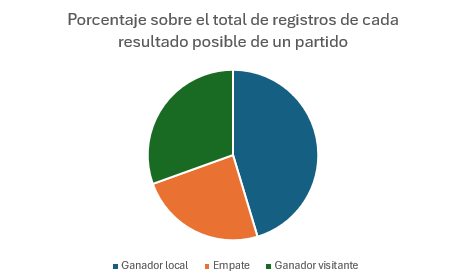
\includegraphics[scale=0.75]{svg/grafico-circular-ganador.png}
    \caption{Gráfico circular con el porcentaje sobre el total de registros de cada resultado posible de un partido. }
    \label{fig:grafico-circular-ganador}
\end{figure}







En segundo lugar, en la Tabla \ref{fig:distribucion-local} se puede ver la distribución de los registros para la clase del número de goles del local en el partido. Aquí se puede ver que lo más habitual es que marque un gol el local.
\begin{table}[]
    \centering
    \begin{tabular}{|l|l|l|}
    \hline
    \rowcolor[HTML]{C0C0C0} 
    Goles marcados por el local & Cuenta & Porcentaje sobre el total \\ \hline
    0     & 1057   & 21,93                     \\ \hline
    1            & 1533   & 31,80                     \\ \hline
    2 & 1221   & 25,33                     \\ \hline
    3 & 615   & 12,76                     \\ \hline
    4 & 244   & 5,06                    \\ \hline
    5 & 113   & 2,34                     \\ \hline
    6 & 29   & 0,60                     \\ \hline
    7 & 4   & 0,08                     \\ \hline
    8 & 3   & 0,06                     \\ \hline
    9 & 1   & 0,02                     \\ \hline
    \end{tabular}
    \caption{Distribución de los registros para la clase del número de goles del local en el partido. }
    \label{fig:distribucion-local}
\end{table}

En la Figura \ref{fig:distribucion-local} se ve de manera gráfica mediante un gráfico circular cómo se reparten las proporciones del número de goles anotados por el local en un partido sobre el total de registros.
\begin{figure}[H]
    \centering
    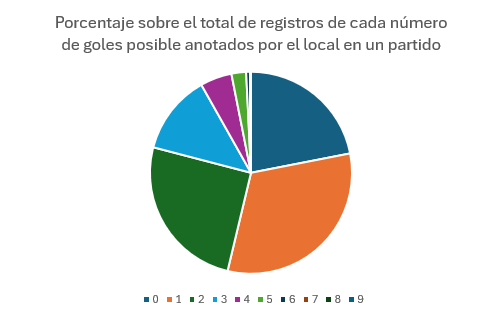
\includegraphics[scale=0.75]{svg/grafico-circular-local.png}
    \caption{Gráfico circular con el porcentaje sobre el total de registros de cada número de goles anotados por el local posible. }
    \label{fig:grafico-circular-local}
\end{figure}






En tercer lugar, en la Tabla \ref{fig:distribucion-visitante} se puede ver la distribución de los registros para la clase del número de goles del visitante en el partido. Aquí se puede ver que lo más habitual es que marque un gol o no anote el equipo visitante.
\begin{table}[]
    \centering
    \begin{tabular}{|l|l|l|}
    \hline
    \rowcolor[HTML]{C0C0C0} 
    Goles marcados por el visitante & Cuenta & Porcentaje sobre el total \\ \hline
    0     & 1480   & 30,71                     \\ \hline
    1            & 1674   & 34,73                     \\ \hline
    2 & 995   & 20,64                     \\ \hline
    3 & 421   & 8,73                     \\ \hline
    4 & 181   & 3,76                    \\ \hline
    5 & 49   & 1,02                     \\ \hline
    6 & 18   & 0,37                     \\ \hline
    7 & 1   & 0,02                     \\ \hline
    8 & 0   & 0,00                     \\ \hline
    9 & 1   & 0,02                     \\ \hline
    \end{tabular}
    \caption{Distribución de los registros para la clase del número de goles del visitante en el partido. }
    \label{fig:distribucion-visitante}
\end{table}

En la Figura \ref{fig:grafico-circular-visitante} se ve de manera gráfica mediante un gráfico circular cómo se reparten las proporciones del número de goles anotados por el visitante en un partido sobre el total de registros.
\begin{figure}[H]
    \centering
    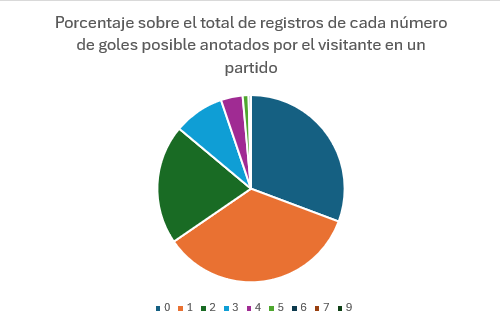
\includegraphics[scale=0.75]{svg/grafico-circular-visitante.png}
    \caption{Gráfico circular con el porcentaje sobre el total de registros de cada número de goles anotados por el visitante posible. }
    \label{fig:grafico-circular-visitante}
\end{figure}

\section{Implementación}
El código del proyecto se ha ejecutado en una máquina virtual proporcionada por la Escuela y en Google Colaboratory.
Todo el código del proyecto se ha dividido en diferentes carpetas. A continuación se detalla la finalidad de cada una estas carpetas y sus archivos:
\begin{itemize}
    \item \textbf{Carpeta \textit{``scraping''}:} en esta carpeta hay diferentes archivos en Python que se encargan de realizar el \textit{scraping} para extraer los datos de la web. Estos archivos están numerados por orden ya que cada uno se encarga de extraer unos determinados datos de una entidad. La descripción de la finalidad de cada uno de estos archivos es la siguiente:
          \begin{itemize}
              \item \textbf{Constantes.py:} en él se definen las ligas y temporadas sobre las que se quieren extraer los datos.
              \item \textbf{EjecuccionGlobal.py:} este el fichero que se debe ejecutar para obtener los datos de las ligas y temporadas definidas en el anterior fichero. Este archivo se encarga de ejecutar sucesivamente cada uno de los archivos que se comentan a continuación e ir extrayendo los datos correspondientes.
              \item \textbf{1ObtencionEquiposLiga.py:} al ejecutarlo se extraen los datos de los equipos en las ligas y temporadas definidas en el fichero de constantes.
              \item \textbf{2ObtencionPlantillasEquipos.py:} al ejecutarlo se extraen los datos de los jugadores en los equipos previamente obtenidos en las ligas y temporadas definidas en el fichero de constantes.
              \item \textbf{3ObtencionPartidos.py:} al ejecutarlo se extraen los datos de los partidos en las ligas y temporadas definidas en el fichero de constantes.
              \item \textbf{4ObtencionDatosJugadoresPartido.py:} al ejecutarlo se extraen los datos de los jugadores de los partidos en las ligas y temporadas definidas en el fichero de constantes.
              \item \textbf{5ObtencionDatosPartidoJugado.py:} al ejecutarlo se extraen los datos más concretos y detallados de los partidos en las ligas y temporadas definidas en el fichero de constantes.
              \item \textbf{6ObtencionIndicadoresEquiposHistorico.py:} al ejecutarlo se extraen los datos de los indicadores de los equipos en cada uno de los partidos en las ligas y temporadas definidas en el fichero de constantes.
              \item \textbf{7PreparacionModelo.py:} al ejecutarlo se transforman los datos de los indicadores de cada partido en el formato adecuado para que se puedan utilizar para entrenar los modelos.
          \end{itemize}
    \item \textbf{Carpeta ``modelos'':} en esta carpeta se encuentran los archivos que se encargan de entrenar los modelos. Cada archivo se asocia al entrenamiento de un modelo y el fichero con los datos con los que se entrenan los modelos se llama ``datosModelo'' y está en formato csv.
    \item \textbf{Carpeta ``csv'':} en esta carpeta se encuentran los datos extraídos mediante los archivos que realizan el \textit{scraping}. Los archivos se agrupan por competición y temporada, de manera que se crean varias carpetas donde cada una contiene varios csv con los datos extraídos para cada una de las entidades previamente comentadas para esa temporada y liga.
    \item \textbf{Carpeta ``analisis-datos'':} en esta carpeta se encuentran los archivos que se encargan de realizar el análisis previo de los datos antes de entrenar los modelos para detectar patrones. En esta carpeta se pueden apreciar dos archivos ipynb que son:
          \begin{itemize}
              \item \textbf{extraccionDatosEquipo.ipynb}: este fichero se encarga de extraer del último partido de cada equipo en una temporada, los valores de sus indicadores en general. De entrada, este fichero recibe el csv con los datos de la entidad ``indicadoresEquipoHistoricoModelo'', el csv con los partidos y el csv con los equipos para una liga y temporada determinada. De salida proporciona para cada equipo, su valor en cada uno de los indicadores considerados que son analizados de manera general, es decir, teniendo en cuenta todos los partidos que ha jugado el equipo en la temporada tanto como de local como de visitante.
              \item \textbf{analisisAtributosEquipo.ipynb}: este fichero se encarga de calcular para cada equipo la diferencia de posiciones que existen entre la clasificación por puntos y la clasificación por cada indicador. De entrada, recibe el csv generado por el anterior fichero con los datos de cada indicador para cada equipo en una temporada y liga. De salida genera un csv donde para cada equipo y cada indicador, se recoge el número de posiciones que difiere la posición de ese equipo en la clasificación por puntos y la posición de ese equipo en la clasificación por ese indicador.
          \end{itemize}
\end{itemize}


\section{Proceso de elección de los mejores modelos}
\subsection{Modelos con algoritmos de \textit{machine learning}}
Con los datos obtenidos, se han entrenado diferentes algoritmos de \textit{machine learning} de los comentados en la Sección \ref{machine-learning} con los conceptos teóricos y redes neuronales variando su estructura. Para cada uno de los algoritmos comentados de \textit{machine learning}, se calcula el valor de la exactitud para el modelo entrenado con los mejores parámetros obtenidos tras aplicar su optimización.

En este caso, para los algoritmos de \textit{machine learning} cabe recordar que los algoritmos que se iban a evaluar eran los árboles de decisión, máquinas de vectores de soporte, k-vecinos más cercanos, \textit{gradient boosting machines}, bosques aleatorios y Gaussian Naive Bayes. Al entrenar estos algoritmos se utiliza el conjunto de datos después de realizar las operaciones de limpieza y transformación previamente comentadas.

Por otro lado, en el Apéndice \ref{combinaciones-parametros} se pueden encontrar todos los valores diferentes que se han probado para optimizar los parámetros de los modelos creados con \textit{machine learning}.








En la Tabla \ref{table:exactitud-ganador} se puede ver qué valor sobre la métrica evaluada han obtenido los diferentes modelos creados utilizando algoritmos de \textit{machine learning} con la mejor combinación de parámetros para cada algoritmo para el problema de predecir el ganador del partido sobre el conjunto de prueba.




\begin{table}[]
    \centering
    \begin{tabularx}{\textwidth}{|l|>{\raggedright\arraybackslash}X|l|}
        \hline
        \rowcolor[HTML]{C0C0C0}
        Algoritmo              & Mejores parámetros                                               & Exactitud (\textit{Accuracy}) del modelo creado \\ \hline
        Árbol de decisión      & ``max depth'': 3, ``min samples split'': 2                               & 0,507                                  \\ \hline
        SVM                    & ``C'': 10, ``gamma'': 0,001, ``kernel'': rbf                                 & 0,532                                  \\ \hline
        K-vecinos más cercanos & ``n neighbors'': 7, ``p'': 2, ``weights'': uniform                           & 0,485                                  \\ \hline
        GBM                   & ``learning rate'': 0,01, ``max depth'': 3, ``n estimators'': 50              & 0,494                                  \\ \hline
        Bosques aleatorios     & ``max depth'': 10, ``min samples split'': 10, ``n estimators'': 100          & 0,535                                  \\ \hline
        Gaussian Naive Bayes   & ``var smoothing'': 1e-09                                             & 0,476                                  \\ \hline
    \end{tabularx}
    \caption{Valor de la exactitud para cada uno de los modelos entrenados utilizando algoritmos de \textit{machine learning} para predecir el ganador del partido.}
    \label{table:exactitud-ganador}
\end{table}

En este caso los dos algoritmos con mejor valor en la métrica evaluada son los bosques aleatorios y SVM, siendo ligeramente mejor el modelo que utiliza los bosques aleatorios. Para confirmar esto se han utilizado el resto de las métricas que se definieron en la parte teórica para evaluar la calidad de los modelos, para de esta forma terminar de confirmar si el modelo con los bosques aleatorios es mejor y en ese caso seguir profundizando para continuar depurando sus parámetros. En la Tabla \ref{table:resto-metricas-ganador} se muestran el resto de valores de las métricas sobre los modelos entrenados con estos algoritmos.

\begin{table}[]
    \centering
    \begin{tabular}{|l|l|l|}
        \hline
        \rowcolor[HTML]{C0C0C0}
        Métrica/Algoritmo   & Bosques aleatorios & SVM  \\ \hline
        Precisión & 0,48               & 0,42 \\ \hline
        Exhaustividad    & 0,54               & 0,53 \\ \hline
        Puntuación F1  & 0,46               & 0,45 \\ \hline
    \end{tabular}
    \caption{Valor del resto de las métricas sobre los dos mejores modelos para predecir el ganador del partido.}
    \label{table:resto-metricas-ganador}
\end{table}

A continuación, en la Figura \ref{fig:matriz-svm-ganador} se ve la matriz de confusión para el modelo entrenado optimizando los parámetros para una SVM y en la Figura \ref{fig:matriz-bosque-ganador} se ve la matriz de confusión para el modelo entrenado optimizando los parámetros para un bosque aleatorio.

\begin{figure}[H]
    \centering
    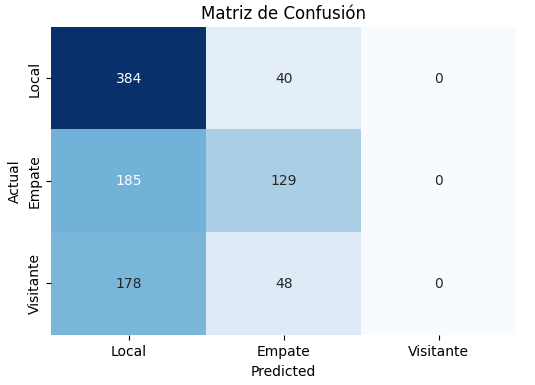
\includegraphics[scale=0.60]{svg/matriz-svm-ganador.png}
    \caption{Matriz de confusión para el modelo entrenado para predecir el ganador del partido utilizando SVM. }
    \label{fig:matriz-svm-ganador}
\end{figure}

\begin{figure}[H]
    \centering
    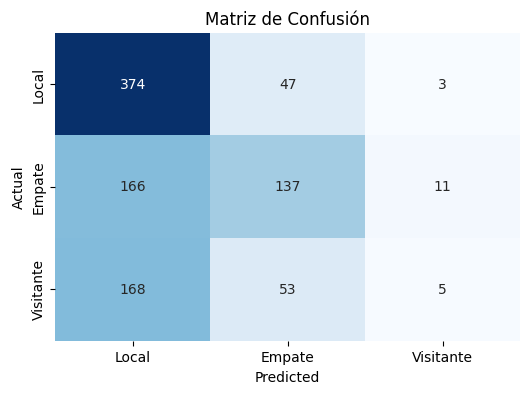
\includegraphics[scale=0.60]{svg/matriz-bosque-ganador.png}
    \caption{Matriz de confusión para el modelo entrenado para predecir el ganador del partido utilizando bosques aleatorios. }
    \label{fig:matriz-bosque-ganador}
\end{figure}


Por lo tanto, para el ganador del partido el modelo que proporciona mejores valores en las métricas evaluadas utiliza el algoritmo de los bosques aleatorios. Por lo tanto, se va a tratar de seguir profundizando y depurando sus parámetros para incrementar aún más su rendimiento. Para ello, se ha vuelto a realizar el proceso de entrenamiento pero en este caso, cambiando los valores posibles de los parámetros a valores más cercanos a los que se acaban de seleccionar con esta primera ejecución. Estos valores son para ``max depth'' 25, 30 y 35, para ``min samples split'' 2, 3, y 4 y para ``n estimators'' 190, 200 y 210. Tras el entrenamiento del modelo con validación cruzada con esta opciones posibles para los parámetros, se ha visto que el modelo finalmente creado utilizando bosques aleatorios tiene de parámetros ``max depth'': 35, ``min samples split'': 3, ``n estimators'': 200 y un valor sobre la exactitud de 0,542.














En la Tabla \ref{table:exactitud-local} se puede ver qué valor sobre la métrica evaluada han obtenido los diferentes modelos creados utilizando algoritmos de \textit{machine learning} con la mejor combinación de parámetros para cada algoritmo para el problema de predecir los goles marcados por el equipo local.

\begin{table}[]
    \centering
    \begin{tabularx}{\textwidth}{|l|>{\raggedright\arraybackslash}X|l|}
        \hline
        \rowcolor[HTML]{C0C0C0}
        Algoritmo              & Mejores parámetros                                     & Exactitud (\textit{Accuracy}) del modelo creado \\ \hline
        Árbol de decisión      & ``max depth'': 3, ``min samples split'': 2                     & 0,331                                  \\ \hline
        SVM                    & ``C'': 0,1, ``gamma'': 0,001, ``kernel'': linear                   & 0,341                                  \\ \hline
        K-vecinos más cercanos & ``n neighbors'': 7, ``p: 1, ``weights'': uniform                 & 0,306                                  \\ \hline
        GBM                    & ``learning rate'': 0,01, ``max depth'': 4, ``n estimators'': 50    & 0,315                                  \\ \hline
        Bosques aleatorios     & ``max depth'': 10, ``min samples split'': 2, ``n estimators'': 200 & 0,348                                  \\ \hline
        Gaussian Naive Bayes   & ``var smoothing'': 1e-09                                  & 0,263                                  \\ \hline
    \end{tabularx}
    \caption{Valor de la exactitud para cada uno de los modelos entrenados utilizando algoritmos de \textit{machine learning} para predecir los goles del local.}
    \label{table:exactitud-local}
\end{table}

En este caso los dos algoritmos con mejor valor en la métrica evaluada son los bosques aleatorios y SVM, al igual que el caso anterior, siendo ligeramente mejor el modelo que utiliza los bosques aleatorios. Para confirmar esto se han utilizado el resto de las métricas que se definieron en la parte teórica para evaluar la calidad de los modelos, para de esta forma terminar de confirmar si el modelo con los bosques aleatorios es mejor y en ese caso seguir profundizando para continuar depurando sus parámetros. En la Tabla \ref{table:resto-metricas-local} se muestran el resto de valores de las métricas sobre los modelos entrenados con estos algoritmos.

\begin{table}[]
    \centering
    \begin{tabular}{|l|l|l|}
        \hline
        \rowcolor[HTML]{C0C0C0}
        Métrica/Algoritmo   & Bosques aleatorios & SVM  \\ \hline
        Precisión & 0,34               & 0,41 \\ \hline
        Exhaustividad    & 0,35               & 0,34 \\ \hline
        Puntuación F1  & 0,30               & 0,24 \\ \hline
    \end{tabular}
    \caption{Valor del resto de las métricas sobre los dos mejores modelos para predecir los goles del local.}
    \label{table:resto-metricas-local}
\end{table}

A continuación, en la Figura \ref{fig:matriz-svm-local} se ve la matriz de confusión para el modelo entrenado optimizando los parámetros para una SVM y en la Figura \ref{fig:matriz-bosque-local} se ve la matriz de confusión para el modelo entrenado optimizando los parámetros para un bosque aleatorio.

\begin{figure}[H]
    \centering
    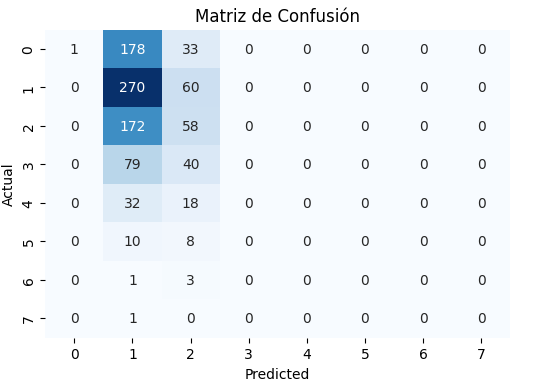
\includegraphics[scale=0.60]{svg/matriz-svm-local.png}
    \caption{Matriz de confusión para el modelo entrenado para predecir los goles del local utilizando SVM. }
    \label{fig:matriz-svm-local}
\end{figure}

\begin{figure}[H]
    \centering
    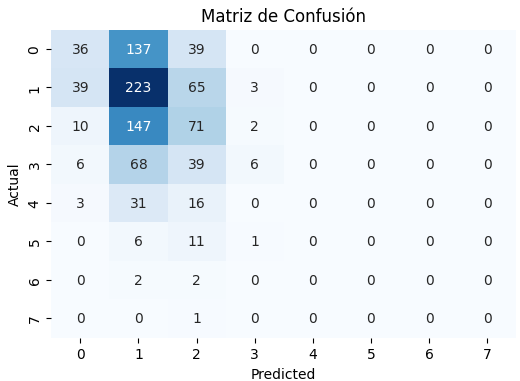
\includegraphics[scale=0.60]{svg/matriz-bosque-local.png}
    \caption{Matriz de confusión para el modelo entrenado para predecir los goles del local utilizando bosques aleatorios. }
    \label{fig:matriz-bosque-local}
\end{figure}


Por lo tanto, para los goles del local el modelo que proporciona mejores valores en las métricas evaluadas utiliza el algoritmo de los bosques aleatorios. Por lo tanto, se va a tratar de seguir profundizando y depurando sus parámetros para incrementar aún más su rendimiento. Para ello, se ha vuelto a realizar el proceso de entrenamiento pero en este caso, cambiando los valores posibles de los parámetros a valores más cercanos a los que se acaban de seleccionar con esta primera ejecución. Estos valores son para ``max depth'' 8, 10 y 12, para ``min samples split'' 2, 3, y 4 y para ``n estimators'' 190, 200 y 210. Tras el entrenamiento del modelo con validación cruzada con esta opciones posibles para los parámetros, se ha visto que el modelo finalmente creado utilizando bosques aleatorios tiene de parámetros ``max depth'': 8, ``min samples split'': 3, ``n estimators'': 200 y un valor sobre la exactitud de 0,349.













En la Tabla \ref{table:exactitud-visitante} se puede ver qué valor sobre la métrica evaluada han obtenido los diferentes modelos creados utilizando algoritmos de \textit{machine learning} con la mejor combinación de parámetros para cada algoritmo para el problema de predecir los goles del visitante.

\begin{table}[]
    \centering
    \begin{tabularx}{\textwidth}{|l|>{\raggedright\arraybackslash}X|l|}
        \hline
        \rowcolor[HTML]{C0C0C0}
        Algoritmo              & Mejores parámetros                                     & Exactitud (\textit{Accuracy}) del modelo creado \\ \hline
        Árbol de decisión      & ``max depth'': 3, ``min samples split'': 2                     & 0,330                                  \\ \hline
        SVM                    & ``C'': 0,1, ``gamma'': 0,001, ``kernel'': linear                   & 0,359                                  \\ \hline
        K-vecinos más cercanos & ``n neighbors'': 7, ``p'': 2, ``weights'': uniform                 & 0,329                                  \\ \hline
        GBM                    & ``learning rate'': 0,01, ``max depth'': 3, ``n estimators'': 50    & 0,336                                  \\ \hline
        Bosques aleatorios     & ``max depth'': 30, ``min samples split'': 2, ``n estimators'': 200 & 0,352                                  \\ \hline
        Gaussian Naive Bayes   & ``var smoothing'': 1e-09                                   & 0,299                                  \\ \hline
    \end{tabularx}
    \caption{Valor de la exactitud para cada uno de los modelos entrenados utilizando algoritmos de \textit{machine learning} para predecir los goles del visitante.}
    \label{table:exactitud-visitante}
\end{table}


En este caso los dos algoritmos con mejor valor en la métrica evaluada son los bosques aleatorios y SVM, al igual que en los casos anteriores, siendo ligeramente mejor el modelo que utiliza los bosques aleatorios. Para confirmar esto se han utilizado el resto de las métricas que se definieron en la parte teórica para evaluar la calidad de los modelos, para de esta forma terminar de confirmar si el modelo con los bosques aleatorios es mejor y en ese caso seguir profundizando para continuar depurando sus parámetros. En la Tabla \ref{table:resto-metricas-visitante} se muestran el resto de valores de las métricas sobre los modelos entrenados con estos algoritmos.

\begin{table}[]
    \centering
    \begin{tabular}{|l|l|l|}
        \hline
        \rowcolor[HTML]{C0C0C0}
        Métrica/Algoritmo   & Bosques aleatorios & SVM  \\ \hline
        Precisión & 0,33               & 0,24 \\ \hline
        Exhaustividad    & 0,35               & 0,36 \\ \hline
        Puntuación F1  & 0,30               & 0,28 \\ \hline
    \end{tabular}
    \caption{Valor del resto de las métricas sobre los dos mejores modelos para predecir los goles del visitante.}
    \label{table:resto-metricas-visitante}
\end{table}

A continuación, en la Figura \ref{fig:matriz-svm-visitante} se ve la matriz de confusión para el modelo entrenado optimizando los parámetros para una SVM y en la Figura \ref{fig:matriz-bosque-visitante} se ve la matriz de confusión para el modelo entrenado optimizando los parámetros para un bosque aleatorio.

\begin{figure}[H]
    \centering
    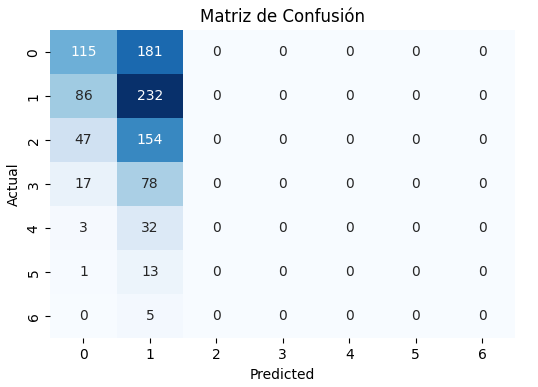
\includegraphics[scale=0.60]{svg/matriz-svm-visitante.png}
    \caption{Matriz de confusión para el modelo entrenado para predecir los goles del visitante utilizando SVM. }
    \label{fig:matriz-svm-visitante}
\end{figure}

\begin{figure}[H]
    \centering
    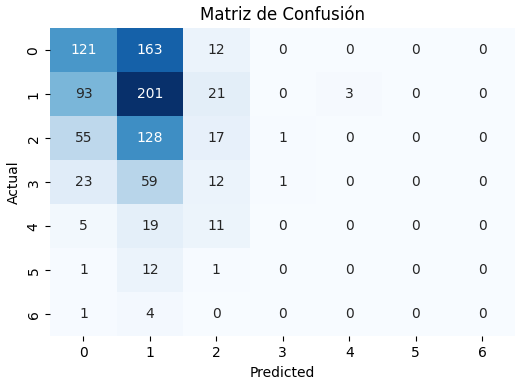
\includegraphics[scale=0.60]{svg/matriz-bosque-visitante.png}
    \caption{Matriz de confusión para el modelo entrenado para predecir los goles del visitante utilizando bosques aleatorios. }
    \label{fig:matriz-bosque-visitante}
\end{figure}


Por lo tanto, para los goles del visitante el modelo que proporciona mejores valores en las métricas evaluadas utiliza el algoritmo de los bosques aleatorios. Por lo tanto, se va a tratar de seguir profundizando y depurando sus parámetros para incrementar aún más su precisión. Para ello, se ha vuelto a realizar el proceso de entrenamiento pero en este caso, cambiando los valores posibles de los parámetros a valores más cercanos a los que se acaban de seleccionar con esta primera ejecución. Estos valores son para ``max depth'' 25, 30 y 35, para ``min samples split'' 2, 3, y 4 y para ``n estimators'' 190, 200 y 210. Tras el entrenamiento del modelo con validación cruzada con esta opciones posibles para los parámetros, se ha visto que el modelo finalmente creado utilizando bosques aleatorios tiene de parámetros ``max depth'': 30, ``min samples split'': 2, ``n estimators'': 200 y un valor sobre la exactitud de 0,352.





\subsection{Modelos con redes neuronales}
Por otra parte, la otra opción que se iban a implementar eran las redes neuronales. En estos casos, para las redes neuronales, en la Tabla \ref{table:parametros-redes}, se establecen los parámetros que se han optimizado sobre estas redes neuronales y los valores diferentes que podían tomar.

\begin{table}[]
    \centering
    \begin{tabular}{|l|l|}
        \hline
        \rowcolor[HTML]{C0C0C0}
        Parámetro       & Valores diferentes \\ \hline
        Tipo de red     & 1,2,3,4,5,6        \\ \hline
        Tamaño de lote & 16,48,80           \\ \hline
        Épocas          & 20,50,80           \\ \hline
        Optimizador     & ``Adam'', ``SGD'', ``RMSProp'' \\ \hline
        \textit{Callbacks}       & Si, No             \\ \hline
    \end{tabular}
    \caption{Parámetros a evaluar en las redes neuronales.}
    \label{table:parametros-redes}
\end{table}




Previo a esta elección de parámetros, se realizó un filtrado eliminando opciones que no tenían
repercusión sobre la exactitud de los modelos. Por ejemplo, se redujeron los valores del tamaño de lote y las épocas
a analizar a tres valores diferentes, ya que no existía mucha diferencia entre estos valores. Por otro lado, se vió que cambiando la función de pérdida no se observaban cambios significativos en las métricas de los modelos entrenados, por lo tanto como función de pérdida se estableció por defecto \textit{categorical crossentropy} y de esta forma también se evitaban evaluar más combinaciones de parámetros. Para el tamaño del lote se han establecido valores en un rango amplio y al igual que con las épocas, se han reducido los valores a tres opciones distintas.

A continuación, se detalla la estructura de cada uno de los tipos diferentes de red que se han evaluado:
\begin{itemize}
    \item \textbf{Tipo de red 1:} consta de tres capas densas. La primera capa es una capa densa con 128 unidades y utilizando como función de activación ``ReLU'', seguida de una capa de \textit{BatchNormalization} y una capa de \textit{Dropout} con una tasa del 30\% para ayudar a prevenir el sobreajuste. La segunda capa es otra capa densa en este caso con 64 unidades y tambien como función de activación ``ReLU'', seguida por una capa de \textit{BatchNormalization} y otra capa de \textit{Dropout} del 30\%. La capa de salida finalmente es una capa densa con el número de unidades según el problema para el que sea y función de activación ``softmax'', que es la que se utiliza para problemas de clasificación multiclase.
    \item \textbf{Tipo de red 2:} consta de cuatro capas densas. La primera capa es una capa densa con 256 unidades y utilizando como función de activación ``ReLU'', seguida de una capa de \textit{BatchNormalization} y una capa de \textit{Dropout} con una tasa del 40\% para evitar el sobreajuste. La segunda capa es otra capa densa con 128 unidades e igualmente con la función de activación ``ReLU'', seguida por otra capa de \textit{BatchNormalization} y otra capa de \textit{Dropout} del 40\%. La tercera capa es una capa densa con 64 unidades y con función de activación ``ReLU'', seguida además de una capa de \textit{BatchNormalization} y una capa de \textit{Dropout} del 40\%. La capa de salida es una capa densa con el número de unidades según el problema para el que sea y función de activación ``softmax'', que es la más adecuada para tareas de clasificación multiclase.
    \item \textbf{Tipo de red 3:} consta de cuatro capas densas. La primera capa es una capa densa con 256 unidades y que utiliza como función de activación ``ReLU'', que incluye un \textit{bias initializer} de 0,1 y \textit{bias regularizer} L2 con un factor de 0,01, seguida de una capa de \textit{BatchNormalization} y una capa de \textit{Dropout} con una tasa del 40\%. La segunda capa es otra capa densa con 128 unidades, también con función de activación ``ReLU'', el mismo \textit{bias initializer} y \textit{regularizer}, seguida también por una capa de \textit{BatchNormalization} y otra capa de \textit{Dropout} del 40\%. La tercera capa densa tiene 64 unidades con los mismos valores de inicialización y regularización de bias, seguida por una capa de \textit{BatchNormalization} y una capa de \textit{Dropout} del 40\%. La capa de salida para finalizar es una capa densa con el número de unidades según el problema para el que sea, función de activación ``softmax'', \textit{bias initializer} de 0,1 y \textit{bias regularizer} L2 con un factor de 0,01, útil para tareas de clasificación multiclase.
    \item \textbf{Tipo de red 4:} consta de cuatro capas densas. La primera capa es una capa densa con 256 unidades y que utiliza la función de activación ``ReLU'', que aplica un \textit{kernel initializer} ``He normal'' y un \textit{kernel regularizer} L2 con un factor de 0,01, seguida de una capa de \textit{BatchNormalization} y una capa de \textit{Dropout} con una tasa del 40\%. La segunda capa es otra capa densa con 128 unidades y activación ``ReLU'', donde también se aplica un \textit{kernel initializer} ``He normal'' y \textit{kernel regularizer} L2, seguida de una capa de \textit{BatchNormalization} y una capa de \textit{Dropout} del 40\%. La tercera capa densa tiene 64 unidades, también con \textit{kernel initializer} ``He normal'' y \textit{kernel regularizer} L2, seguida de una capa de \textit{BatchNormalization} y una capa de \textit{Dropout} del 40\%. La capa de salida es una capa densa con el número de unidades según el problema para el que sea, función de activación ``softmax'', \textit{kernel initializer} ``He normal'' y \textit{kernel regularizer} L2 con un factor de 0,01.
    \item \textbf{Tipo de red 5:} consta de tres capas densas. La primera capa es una capa densa con 256 unidades y que aplica de función de activación ``ReLU'', que utiliza un \textit{kernel initializer} ``He normal'' y un \textit{bias initializer} constante de 0,1, además de \textit{kernel} y \textit{bias regularizer} L2 con un factor de 0,01 para ambos, seguida de una capa de \textit{BatchNormalization} y una capa de \textit{Dropout} con una tasa del 40\%. La segunda capa es otra capa densa con 128 unidades y aplicando funcion de activación ``ReLU'', que también emplea un \textit{kernel initializer} ``He normal'', \textit{bias initializer} de 0,1 y \textit{bias regularizer} L2, seguida de una capa de \textit{BatchNormalization} y una capa de \textit{Dropout} del 40\%. La capa de salida es una capa densa con el número de unidades según el problema para el que sea, función de activación ``softmax'', \textit{kernel initializer} ``He normal'', \textit{bias initializer} de 0,1 y tanto Bias como \textit{kernel regularizer} L2.
    \item \textbf{Tipo de red 6:} consta de cinco capas densas, cada una seguida de una capa de \textit{BatchNormalization} y una capa de \textit{Dropout} con una tasa del 50\% para evitar el sobreajuste. La primera capa densa tiene 512 unidades y aplica la función de activación ``ReLU'', la segunda capa densa tiene 256 unidades y tambien aplica activación ``ReLU'', la tercera capa densa tiene 128 unidades y al igual que las anteriores aplica activación ``ReLU'', la cuarta capa densa tiene 64 unidades tambien aplicando activación ``ReLU'', y la quinta capa densa tiene 32 unidades con activación ``ReLU''. La capa de salida es una capa densa con el número de unidades según el problema para el que sea y función de activación ``softmax''.

\end{itemize}


Donde se comenta en la estructura de estas redes sobre que la capa de salida es una capa densa con el número de unidades según el problema para el que sea, esto se refiere a que en este proyecto se consideran tres problemas de clasificación multiclase. El primer problema es evaluar el ganador de los partidos. Las redes neuronales que se entrenen para este problema tendrán la estructura comentada para los anteriores tipos pero sin embargo, en la capa de salida habrá tres unidades, ya que la clase puede tener tres opciones diferentes. Las opciones son que gana el local, que gana el visitante o que el partido finaliza en empate.

Para los otros problemas, donde se pretende predecir el número de goles de tanto el equipo local como el visitante, las variables a predecir en ambos casos cuentan con diez combinaciones posibles. Estas diez combinaciones son el número de goles del equipo en cuestión, que puede ir desde cero goles a nueve goles. Se ha decidido establecer este rango ya que en los datos obtenidos, todos los goles marcados por los equipos en los partidos obtenidos se encuentran en este rango. Por lo tanto, al entrenar estos tipos de redes neuronales comentadas para estos problemas, en estos casos, la capa de salida debe tener diez unidades.

Con estas combinaciones de parámetros, se pueden obtener 324 combinaciones diferentes que son las que
se han evaluado para crear los mejores modelos para predecir tanto el resultado del partido, los
goles del local y los goles del visitante. Por lo tanto, con los datos obtenidos, para cada
combinación de parámetros, se entrena una red neuronal y se evalúa su exactitud. Finalmente se
obtienen los parámetros que se utilizaron en la red neuronal que mejor exactitud ha obtenido. Este
proceso se realiza para predecir el ganador del partido, los goles del equipo local y los goles del
equipo visitante, obteniendo tres combinaciones de parámetros que se comentan a continuación.

Para optimizar este proceso, se van evaluando las combinaciones diferentes de parámetros por paquetes, pivotando alrededor del optimizador. Es decir, en primer lugar se entrenan los modelos y se calculan sus métricas utilizando todas las combinaciones de parámetros pero manteniendo el optimizador ``adam''. Después se realiza lo mismo manteniendo el optimizador ``SGD'' y finalmente manteniendo el optimizador ``RMSprop''. De esta forma las 324 combinaciones distintas se evalúan en tres paquetes de 108 combinaciones distintas cuyo tiempo de ejecución es bastante menor.

Por otro lado, en las primeras pruebas se ha visto que la calidad de los modelos al variar el número de épocas entre 20, 50 y 80 apenas varia, pero sin embargo, el tiempo utilizado por los modelos con 80 épocas es considerablemente mayor en los otros modelos. Por lo tanto, se ha decidido acotar las opciones de este parámetro en valores más pequeños que tengan menores tiempos de ejecución pero donde el rendimiento no se vea afectado. Los valores finalmente evaluados para este parámetro han sido 20, 30 y 40.

En la Tabla \ref{table:exactitud-redes-ganador} se ven las diez redes neuronales con diferentes combinaciones de parámetros con mayor valor de exactitud para el problema de predecir el ganador del partido.

\begin{table}[]
    \centering
    \begin{tabular}{|l|l|l|l|l|l|l|}
        \hline
        \rowcolor[HTML]{C0C0C0}
        Ranking & Tipo de red & Optimizador & Épocas & Tamaño de lote & \textit{Callbacks} & Exactitud \\ \hline
        1                & 5           & ``SGD''         & 20     & 48         & No        & 0,560     \\ \hline
        2                & 1           & ``Adam''        & 50     & 80         & No        & 0,558     \\ \hline
        3                & 2           & ``Adam''        & 80     & 16         & Si        & 0,557     \\ \hline
        4                & 5           & ``Adam''        & 20     & 16         & No        & 0,556     \\ \hline
        5                & 1           & ``SGD''         & 50     & 16         & No        & 0,554     \\ \hline
        6                & 1           & ``Adam''        & 80     & 16         & No        & 0,553     \\ \hline
        7                & 2           & ``Adam''        & 80     & 16         & No        & 0,552     \\ \hline
        8                & 2           & ``Adam''        & 20     & 80         & No        & 0,551     \\ \hline
        9                & 1           & ``SGD''         & 50     & 16         & Si        & 0,551     \\ \hline
        10               & 2           & ``Adam''        & 20     & 48         & No        & 0,549     \\ \hline
    \end{tabular}
    \caption{Valor de la exactitud para las diez estructuras de redes neuronales que mayores valores han proporcionado en esa métrica para predecir el ganador del partido.}
    \label{table:exactitud-redes-ganador}
\end{table}



Por lo tanto, respecto al ganador del partido, finalmente se ha seleccionado como el mejor modelo con mayor
exactitud, una red neuronal con Tensorflow, en la que se han seleccionado de entre las 324
combinaciones posibles de parámetros, una estructura con 3 capas que corresponde con el tipo de red 5 previamente definido, con descenso de gradiente
estocástico como optimizador (``SGD''), con entropía cruzada categórica como función de pérdida,
entrenada en 20 épocas con un tamaño de lote de 48 que no incorpora \textit{callbacks}. Esta red ha
obtenido una exactitud sobre el conjunto de prueba del 0,560.



En la Tabla \ref{table:exactitud-redes-local} se ven las diez redes neuronales con diferentes combinaciones de parámetros con mayor valor de exactitud para el problema de predecir los goles del local en el partido.

\begin{table}[]
    \centering
    \begin{tabular}{|l|l|l|l|l|l|l|}
        \hline
        \rowcolor[HTML]{C0C0C0}
        Ranking & Tipo de red & Optimizador & Épocas & Tamaño de lote & \textit{Callbacks} & Exactitud \\ \hline
        1                & 6           & ``SGD''         & 20     & 80         & No        & 0,370     \\ \hline
        2                & 2           & ``SGD''        & 80     & 48         & Si        & 0,368     \\ \hline
        3                & 3           & ``SGD''        & 80     & 48         & No        & 0,366     \\ \hline
        4                & 3           & ``SGD''        & 80     & 48         & No        & 0,364     \\ \hline
        5                & 6           & ``SGD''         & 50     & 48         & Si        & 0,363     \\ \hline
        6                & 3           & ``SGD''        & 50     & 80         & No        & 0,362     \\ \hline
        7                & 2           & ``SGD''        & 50     & 16         & No        & 0,361     \\ \hline
        8                & 6           & ``SGD''        & 20     & 48         & Si        & 0,361     \\ \hline
        9                & 3           & ``SGD''         & 80     & 16         & Si        & 0,359     \\ \hline
        10               & 3           & ``SGD''        & 50     & 80         & Si        & 0,359     \\ \hline
    \end{tabular}
    \caption{Valor de la exactitud para las diez estructuras de redes neuronales que mayores valores han proporcionado en esa métrica para predecir los goles del local en el partido.}
    \label{table:exactitud-redes-local}
\end{table}


Respecto a los goles del local, finalmente se ha seleccionado como el mejor modelo con mayor
precisión, una red neuronal con Tensorflow, en la que se han seleccionado de entre las 108
combinaciones posibles de parámetros, una estructura con 5 capas que corresponde con el tipo de red 6, con descenso de gradiente
estocástico como optimizador (``SGD''), con entropía cruzada categórica como función de pérdida,
entrenada en 20 épocas con un tamaño de lote de 80 que no incorpora \textit{callbacks}. Esta red ha
obtenido una exactitud sobre el conjunto de prueba del 0,370.

En la Tabla \ref{table:exactitud-redes-visitante} se ven las diez redes neuronales con diferentes combinaciones de parámetros con mayor valor de exactitud para el problema de predecir los goles del visitante en el partido.

\begin{table}[]
    \centering
    \begin{tabular}{|l|l|l|l|l|l|l|}
        \hline
        \rowcolor[HTML]{C0C0C0}
        Ranking & Tipo de red & Optimizador & Épocas & Tamaño de lote & \textit{Callbacks} & Exactitud \\ \hline
        1                & 4           & ``Adam''         & 20     & 80         & No        & 0,383     \\ \hline
        2                & 2           & ``Adam''        & 50     & 16         & No        & 0,376     \\ \hline
        3                & 6           & ``Adam''        & 20     & 48         & Si        & 0,374     \\ \hline
        4                & 2           & ``SGD''        & 50     & 80         & No        & 0,374     \\ \hline
        5                & 1           & ``SGD''         & 80     & 16         & No        & 0,374     \\ \hline
        6                & 4           & ``SGD''        & 50     & 16         & Si        & 0,374     \\ \hline
        7                & 1           & ``Adam''        & 80     & 48         & Si        & 0,371     \\ \hline
        8                & 1           & ``Adam''        & 20     & 48         & No        & 0,370     \\ \hline
        9                & 4           & ``SGD''         & 80     & 80         & No        & 0,370     \\ \hline
        10               & 2           & ``SGD''        & 50     & 48         & No        & 0,368     \\ \hline
    \end{tabular}
    \caption{Valor de la exactitud para las diez estructuras de redes neuronales que mayores valores han proporcionado en esa métrica para predecir los goles del visitante en el partido.}
    \label{table:exactitud-redes-visitante}
\end{table}

Respecto a los goles del visitante, finalmente se ha seleccionado como el mejor modelo con mayor
precisión, una red neuronal con Tensorflow, en la que se han seleccionado de entre las 324
combinaciones posibles de parámetros, una estructura con 4 capas que corresponde con el tipo de red 4, con ``adam'' como optimizador,
con entropía cruzada categórica como función de pérdida, entrenada en 20 épocas con un tamaño
de lote de 80 que no incorpora \textit{callbacks}. Esta red ha obtenido una exactitud sobre el conjunto
de prueba del 0,383.

La exactitud de los modelos sobre los goles de los equipos pueden parecer bajas pero se debe
tener en cuenta, que predecir el número de goles exacto de un equipo es más complejo, ya que
este valor puede tomar muchos valores diferentes.



\subsection{Importancia de los indicadores en los modelos.}

La importancia de cada variable al entrenar un modelo de una red neuronal con TensorFlow se refiere a la medida en que cada característica del conjunto de datos de entrada contribuye al rendimiento del modelo. Determinar esta importancia para cada atributo es fundamental para entender cómo el modelo toma sus decisiones y qué variables son las que tienen un mayor impacto en las predicciones. Determinar las variables más importantes en los modelos ayuda a mejorar su eficiencia, eliminar datos que pueden ser redundantes y comprender de mejor manera lo que se pretende predecir.


En la Tabla \ref{table:importancia-indicadores-ganador} se muestran los 15 indicadores que mayor importancia tienen ordenando de mayor a menor por este valor en el modelo que se ha creado con una red neuronal para predecir el ganador del partido, destacando los indicadores asociados a la gestión de los jugadores que realizan los equipos.


\begin{table}[]
    \begin{tabularx}{\textwidth}{|l|>{\raggedright\arraybackslash}X|l|}
    \hline
    \rowcolor[HTML]{C0C0C0} 
    Posición & Indicador & Importancia \\ \hline
    1        &    porcentaje del local de más 2,5 goles encajados en sitio
    &    0,0067         \\ \hline
    2        &     \textbf{proporción del local de cambios de goleadores en sitio}      &    0,0067         \\ \hline
    3        &    porcentaje del local de partidos empatados en general       &   0,0067          \\ \hline
    4        &     proporción del local de córneres en contra en sitio      &     0,0065        \\ \hline
    5        &    porcentaje del visitante de más 1,5 goles en general       &    0,0065         \\ \hline
    6        &    proporción del local de goles totales en sitio       &   0,0065          \\ \hline
    7        &    proporción del local de total tiros en general       &   0,0065          \\ \hline
    8        &    \textbf{proporción del local de cambios de delanteros a defensas en sitio}       &     0,0064        \\ \hline
    9        &   \textbf{proporción del visitante de cambios en general}        &     0,0064        \\ \hline
    10        &   proporción del visitante de total tiros en general        &     0,0064        \\ \hline
    11       &     porcentaje del local de más 0,5 marcados en general      &     0,0063        \\ \hline
    12       &    \textbf{proporción del local de cambios antes descanso en general}       &    0,0063         \\ \hline
    13       &     porcentaje del visitante de más 2,5 en sitio       &    0,0063         \\ \hline
    14       &    \textbf{proporción del visitante de cambios en alineación de defensas en general}       &    0,0063         \\ \hline
    15       &     proporción del local de rojas en general      &    0,0063         \\ \hline

    \end{tabularx}
    \caption{Indicadores con mayor importancia en el modelo creado con una red neuronal para predecir el ganador del partido.}
    \label{table:importancia-indicadores-ganador}
    \end{table}

    


En la Tabla \ref{table:importancia-indicadores-local} se muestran los 15 indicadores que mayor importancia tienen ordenando de mayor a menor por este valor en el modelo que se ha creado con una red neuronal para predecir los goles anotados por el equipo local, destacando los indicadores asociados a la gestión de los jugadores que realizan los equipos.


\begin{table}[]
    \begin{tabularx}{\textwidth}{|l|>{\raggedright\arraybackslash}X|l|}
    \hline
    \rowcolor[HTML]{C0C0C0} 
    Posición & Indicador & Importancia \\ \hline
    1        &   \textbf{media del local del minuto de los cambios en sitio}&	0,0064        \\ \hline
    2        &      \textbf{proporción del local de cambios en la alineación de defensas en general}&	0,0063         \\ \hline
    3        &    porcentaje del visitante de más 3,5 goles en general&	0,0063         \\ \hline
    4        &    porcentaje del visitante de partidos perdidos en general&	0,0063      \\ \hline
    5        &     proporción del local de amarillas en general&	0,0063        \\ \hline
    6        &    proporción del local de córneres en contra en sitio&	0,0062         \\ \hline
    7        &    \textbf{proporción del visitante de cambios en sitio}&	0,0062         \\ \hline
    8        &    proporción del visitante de total tiros en general&	0,0062     \\ \hline
    9        &   \textbf{proporción del local cambios delanteros a centrocampistas en general}&	0,0062        \\ \hline
    10        &   \textbf{proporción del visitante de cambios de goleadores en sitio}&	0,0062       \\ \hline
    11       &     proporción del visitante de goles encajados en general&	0,0062       \\ \hline
    12       &    porcentaje del local de más 4,5 en sitio&	0,0062        \\ \hline
    13       &     \textbf{proporción del visitante cambios en alineación de delanteros en general}&	0,0062         \\ \hline
    14       &    \textbf{proporción del local cambios en alineación de centrocampistas en general}&	0,0062      \\ \hline
    15       &     porcentaje del local de más 2,5 goles encajados en general&	0,0062      \\ \hline

    \end{tabularx}
    \caption{Indicadores con mayor importancia en el modelo creado con una red neuronal para predecir los goles anotados por el equipo local.}
    \label{table:importancia-indicadores-local}
    \end{table}
    
    
   
En la Tabla \ref{table:importancia-indicadores-visitante} se muestran los 15 indicadores que mayor importancia tienen ordenando de mayor a menor por este valor en el modelo que se ha creado con una red neuronal para predecir los goles anotados por el equipo visitante, destacando los indicadores asociados a la gestión de los jugadores que realizan los equipos.


    \begin{table}[]
        \begin{tabular}{|l|l|l|}
        \hline
        \rowcolor[HTML]{C0C0C0} 
        Posición & Indicador & Importancia \\ \hline
        1        &   porcentaje del visitante de más 0,5 goles encajados en sitio&	0,0103       \\ \hline
        2        &     porcentaje del local más 1,5 goles en sitio&	0,0102     \\ \hline
        3        &     \textbf{proporción del visitante de cambios en sitio}&	0,0101        \\ \hline
        4        &    \textbf{proporción del visitante de cambios en general}&	0,0099      \\ \hline
        5        &     porcentaje del local de más 0,5 goles encajados en sitio&	0,0098       \\ \hline
        6        &    porcentaje del local de más 0,5 goles marcados en general&	0,0097        \\ \hline
        7        &    porcentaje del local de más 0,5 goles marcados en sitio&	0,0096       \\ \hline
        8        &    \textbf{proporción del local de cambios en general}&	0,0095     \\ \hline
        9        &   porcentaje del visitante de más 1,5 goles en sitio&	0,0094       \\ \hline
        10        &   porcentaje del visitante de más 0,5 goles marcados en general&	0,0093      \\ \hline
        11       &     \textbf{proporción del local de cambios en sitio}&	0,0093      \\ \hline
        12       &    proporción del visitante de posesión en sitio&	0,009        \\ \hline
        13       &     porcentaje del local de más 0,5 goles encajados en general&	0,0089        \\ \hline
        14       &   porcentaje del visitante de más 0,5 goles marcados en sitio&	0,0088     \\ \hline
        15       &     porcentaje del visitante de más 0,5 goles encajados en general&	0,0088      \\ \hline
    
        \end{tabular}
        \caption{Indicadores con mayor importancia en el modelo creado con una red neuronal para predecir los goles anotados por el equipo visitante.}
        \label{table:importancia-indicadores-visitante}
        \end{table}
        
        
        
       
        
        
        
        
        
        
        
        
        
        
        
        
        
    
   
    
    
    
    
    
    
    
    
    
    
   






    
    
    
    
    
    
    
    
    
   
    
    
   